\documentclass[a4paper, 10pt, final, garamond]{book}
\usepackage{cours-preambule}

\makeatletter
\renewcommand{\@chapapp}{Chimie -- chapitre}
\makeatother

\hfuzz=5.002pt

% \toggletrue{student}
% \toggletrue{corrige}
% \renewcommand{\mycol}{black}
\renewcommand{\mycol}{gray}

\begin{document}
\setcounter{chapter}{5}

% \settype{enon}
% \settype{solu_prof}
% \settype{solu_stud}

\chapter{\cswitch{Correction du TD}{TD~: oxydorédution}}

\resetQ
\section{Équations bilan d'oxydorédution}
\enonce{%
On s'intéresse aux couples
$\ce{{MnO_4^{-}}_{\rm(aq)}}/\ce{{Mn}^2+_{\rm(aq)}}$,
$\ce{HClO_{\rm(aq)}}/\ce{{Cl_2}_{\rm(aq)}}$ et
$\ce{{Cl_2}_{\rm(g)}}/\ce{Cl^-_{\rm(aq)}}$. On rappelle que $\ce{MnO_4^-}$ est
l'ion permanganate et \ce{HClO} l'acide hypochloreux.
}%

\QR{%
	Écrire et équilibrer les demi-équations de chacun des couples en milieu acide.
}{%
	solu
}%
\QR{%
	Lorsque la réaction est possible, écrire l'équation-bilan de la réaction
	entre~:
	\smallbreak
	\noindent
	\begin{minipage}[c]{.45\linewidth}
		\begin{enumerate}[label=\alph*)]
			\item L'acide hypochloreux et l'ion manganèse~;
			\item l'ion manganèse et l'ion chlorure~;
			\item l'ion manganèse et le dichlore~;
		\end{enumerate}
	\end{minipage}
	\hfill
	\begin{minipage}[c]{.45\linewidth}
		\begin{enumerate}[label=\alph*), start=4]
			\item le permanganate et le dichlore~;
			\item le permanganate et l'ion chlorure~;
			\item le dichlore sur lui-même.
		\end{enumerate}
	\end{minipage}
}{%
	solu
}%

\resetQ
\section{Nombres d'oxydation du chrome}
\enonce{%
	Le chrome \ce{Cr} a pour numéro atomique $Z = 24$, et il est moins
	électronégatif que l'oxygène.
}%
\QR{%
	Donner le \no du chrome au sein des espèces $\ce{Cr_{\rm(s)}}$, \ce{Cr^2+} et
	\ce{Cr^3+}.
}{%
	solu
}%
\QR{%
	Sans représenter les schémas de \textsc{Lewis}, déterminer le \no du chrome
	dans les espèces \ce{CrO4^2-} et \ce{Cr2O7^2-}. On précise qu'il n'y a pas de
	liaison \ce{Cr-Cr} dans le dichromate.
}{%
	solu
}%
\QR{%
	Justifier que \ce{Cr2O7^2-} et \ce{Cr^3+} forment un couple rédox. Identifier
	l'oxydant et le réducteur sans utiliser la demi-équation. Écrire
	\textbf{ensuite} la demi-équation associée, en milieu acide et en milieu
	basique.
}{%
	solu
}%
\QR{%
	Justifier que \ce{CrO4^2-} et \ce{Cr2O7^2-} ne forment pas un couple rédox.
	Montrer qu'il s'agit cependant d'un couple acide-base par écriture d'une
	demi-équation.
}{%
	solu
}%

% TODO: oubli du n.o. du soufre piqué à langevin

\resetQ
\section{Dismutation du dioxyde d'azote}
\enonce{%
En présence d'eau, le dioxyde d'azote $\ce{{NO_2}_{\rm(g)}}$ peut se dismuter
en ions nitrates $\ce{{NO_3}^-_{\rm(aq)}}$ et nitrites
$\ce{{NO_2}^-_{\rm(aq)}}$. Cette réaction produit des protons
$\ce{{H}^+_{\rm(aq)}}$, à l'origine des pluies acides.
}%
\QR{%
Écrire le demi-équations de transfert électronique et la relation de
\textsc{Nernst} pour les deux couples
$\ce{{NO_3^{-}}_{\rm(aq)}}/\ce{{NO_2}}_{\rm(g)}$ ($E_1^\circ = \SI{0.83}{V}$)
et $\ce{{NO_2}_{\rm(g)}/{NO_2^{-}}_{\rm(aq)}}$ ($E_2^\circ = \SI{0.85}{V}$).
}{%
solu
}%
\QR{%
	Justifier à l'aide de diagrammes de prédominance que \ce{NO2} se dismute. On
	choisira $p_{\ce{NO_2}} = \SI{1}{bar}$ et une concentration frontière
	(convention de tracé) de $\SI{1}{mol.L^{-1}}$ à pH nul.
}{%
	solu
}%
\QR{%
	Écrire l'équation bilan de l'équation de dismutation.
}{%
	solu
}%
\QR{%
	Exprimer sa constante d'équilibre $K^\circ$ en fonction des potentiels
	standard et calculer sa valeur numérique.
}{%
	solu
}%

\resetQ
\section{Éthylotest}
\enonce{%
	\noindent
	\begin{minipage}[c]{.20\linewidth}
		\begin{center}
			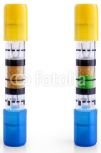
\includegraphics[width=\linewidth]{ethylotest}
		\end{center}
	\end{minipage}
	\hfill
	\begin{minipage}[c]{.75\linewidth}
		Peu après avoir été consommé, l'alcool (éthanol de formule \ce{CH3CH2OH})
		passe dans le sang au niveau de l'intestin grêle. Ensuite, des échanges
		gazeux s'effectuent dans les alvéoles pulmonaires~: le sang se charge en
		dioxygène et se libère du dioxyde de carbone, ainsi que d'une partie de
		l'alcool. Ces vapeurs sont expirées dans l'air avec une concentration en
		alcool \num{2100} fois inférieure à celle du sang. Le seuil limite autorisé
		pour la conduite est de \SI{0.50}{g} d'éthanol par litre de sang.
		\smallbreak
		Les alcootests jetables sont constitués d'un sachet gonflable de capacité
		\SI{1}{L} et d'un tube en verre contenant des cristaux orangés de dichromate
		de potassium \ce{K2Cr2O7} en milieu acide. Ceux-ci se colorent en vert au
		contact de l'alcool.
	\end{minipage}
	\begin{tcb}(data)<lftt>{Données}
		\begin{itemize}
			\item Potentiels standard~: $E^\circ(\ce{Cr_2O_7^2-/Cr^3+}) = E_1^\circ =
				      \SI{1.33}{V}$~; $E^\circ(\ce{CH_3COOH/CH_3CH_2OH}) = E_2^\circ =
				      \SI{0.19}{V}$~;
			\item %
			      \leftcenters{%
				      Masses molaires atomiques~:
			      }{%
				      \begin{tabular}{cccccc}
					      \toprule
					      Élément               & H & C  & O  & K  & Cr
					      \\
					      $M (\si{g.mol^{-1}})$ & 1 & 12 & 16 & 39 & 52
					      \\
					      \bottomrule
				      \end{tabular}
			      }%
		\end{itemize}
	\end{tcb}
}%
\QR{%
	Écrire l'équation de la transformation responsable du changement de couleur.
	Identifier l'espèce oxydée et l'espèce réduite.
}{%
	solu
}%
\QR{%
	Calculer la constante d'équilibre de la réaction. Commenter.
}{%
	solu
}%
\QR{%
	Déterminer la quantité de matière d'alcool expirée par litre d'air, dans
	l'hypothèse d'une alcoolémie atteignant le seuil de \SI{0.50}{g.L^{-1}}
	d'alcool dans un litre de sang.
}{%
	solu
}%
\QR{%
	En déduire la masse de dichromate de potassium devant être placée avant le
	trait de jauge afin que celui-ci indique le seuil limite.
}{%
	solu
}%

\resetQ
\section{Pile argent-zinc}
\enonce{%
On s'intéresse à une pile schématisée par
$\ce{Ag_{\rm(s)}|{Ag}^+_{\rm(aq)}||{Zn}^2+_{\rm(aq)}|Zn_{\rm(s)}}$, avec
$[\ce{Ag+}]_i = c = \SI{0.18}{mol.L^{-1}}$ et $[\ce{Zn^2+}]_i = c' =
	\SI{0.30}{mol.L^{-1}}$. Le compartiment de gauche a un volume $V =
	\SI{100}{mL}$, celui de droite un volume $V' = \SI{250}{mL}$.
\begin{tcb}(data)<lfnt>{Données}
	$E^\circ(\ce{Zn^2+/Zn}) = \SI{-0.76}{V}$ et $E^\circ(\ce{Ag^+/Ag}) =
		\SI{0.80}{V}$.
\end{tcb}
}%
\QR{%
	Déterminer la f.é.m.\ de la pile. Identifier alors l'anode et la cathode par
	un raisonnement sur le trajet des électrons.
}{%
	solu
}%
\QR{%
	Écrire les réactions électrochimiques aux électrodes, puis la réaction de
	fonctionnement qui se produit lorsque la pile débite.
}{%
	solu
}%
\QR{%
	Schématiser le déplacement des porteurs de charge dans chaque partie de la
	pile lorsqu'elle débite du courant.
}{%
	solu
}%
\QR{%
	Déterminer la composition de la pile losqu'elle est usée. Quelle quantité
	d'électricité, en coulombs, a-t-elle débité~?
}{%
	solu
}%

\resetQ
\section{Stabilisation du cuivre I par précipitation}
\enonce{%
	L'objectif de cet exercice est d'étudier la stabilisation du cuivre de
	$\no{\ce{Cu}} = \myRoman{+1}$ par précipitation, qui illustre plus
	généralement l'influence de la précipitation sur l'oxydorédution.
	\begin{tcb}(data)<lfnt>{Données}
		$E^\circ(\ce{Cu^+/Cu}) = E_1^\circ = \SI{0.52}{V}$~;
		$E^\circ(\ce{Cu^2+/Cu^+}) = E_2^\circ = \SI{0.16}{V}$
	\end{tcb}
}%
\QR{%
	Motrer à partir de diagrammes de stabilité que l'ion \ce{Cu^+} est instable.
	Pour simplifier, on prendra \SI{1}{mol.L^{-1}} comme concentration frontière.
	Qu'observe-t-on~?
}{%
	solu
}%
\enonce{%
	Les ions cuivre I forment avec les ions iodure \ce{I^-} le précipité
	$\ce{CuI_{\rm(s)}}$, de produit de solubilité $K_s = \num{e-11}$.
}%
\QR{%
	Écrire l'équation de dissolution du précipité, puis les demi-équations rédox
	pour les couples \ce{CuI/Cu} et \ce{Cu^2+/CuI}.
}{%
	solu
}%
\QR{%
	En déduire la relation de \textsc{Nernst} pour les couples \ce{CuI/Cu} et
	\ce{Cu^2+/CuI} en notant leurs potentiels standard $E_3^\circ$ et $E_4^\circ$,
	respectivement. Exprimer alors $E_3^\circ$ en fonction de $\pk[s]$ et
	$E_1^\circ$ d'une part, puis $E_4^\circ$ en fonction de $\pk[s]$ et
	$E_2^\circ$ d'autre part. Calculer les valeurs numériques.
}{%
	solu
}%
\QR{%
	Expliquer alors en quoi les ions cuivre I sont stabilisés en présence d'ions
	iodure.
}{%
	solu
}%

\resetQ
\section{Dosage colorimétrique en retour}
\enonce{%
	On s'intéresse à un dosage colorimétrique d'une solution de dichromate de
	potassium par les ions fer II en présence d'acide sulfurique, garantissant un
	pH très acide. On donne les potentiels standard
	\[
		E^\circ (\ce{Cr_2O_7^2-/Cr^3+}) = E_1^\circ = \SI{1.33}{V}
		\qet
		E^\circ(\ce{Fe^3+/Fe^2+}) = E_2^\circ = \SI{0.77}{V}
	\]
	En milieu acide, l'ion dichromate est orange et l'ion chrome III est vert,
	alors que l'ion \ce{Fe^2+} est vert pâle et l'ion \ce{Fe^3+} est jaune-orangé.
}%
\QR{%
	Écrire l'équation bilan du titrage rédox direct.
}{%
	solu
}%
\QR{%
	Calculer sa constante d'équilibre. Cette réaction est-elle adaptée à un
	titrage~? Pourquoi est-elle malgré tout peu adaptée à un titrage
	colorimétrique~?
}{%
	solu
}%
\QR{%
	Justifier qu'il serait possible de suivre la réaction par potentiométrie.
	Détreminer le sens du saut de potentiel qui serait observé~: est-il descendant
	ou montant~?
}{%
	solu
}%
\enonce{%
	Pour contourner la difficulté sans montage de potentiométrie, on effectue un
	dosage en retour. Dans un bécher, on verse $V_1 = \SI{4.0}{mL}$ de la solution
	de dichromate de potassium dont on cherche la concentration $c_1$. On y ajoute
	$V_2 = \SI{10.0}{mL}$ d'une solution de sulfate de fer II en milieu
	sulfurique, de concentration $c_2 = \SI{0.10}{mol.L^{-1}}$ et $V_2 -
		\SI{90.0}{mL}$ d'eau. On verse ensuite par une burette une solution de
	permanganate de potassium de concentration $c_3 = \SI{1.0e-2}{mol.L^{-1}}$.
	Une coloration violette, caractéristique du permanganate en solution, apparaît
	lorsque que $V_{3,\eqi} = \SI{12}{mL}$ ont été versés.
}%
\QR{%
	Comment peut-on s'assurer qualitativement que les ions fer II ont bien été
	apportés en excès par rapport au dichromate~?
}{%
	solu
}%
\QR{%
	Écrire l'équation bilan du titrage en retour.
}{%
	solu
}%
\QR{%
	Déterminer la concentration $c_1$ de la solution de dichromate de potassium.
}{%
	solu
}%

\resetQ
\section{Pile à combustible à oxyde solide \hfill \small écrit PT 2015}
\enonce{%
Le principe de la pile à combustible consiste à utiliser du dihydrogène pour
stocker et transporter de l'énergie. Une pile à combustible est un assemblage
de cellules élémentaires, en nombre suffisant pour assurer la production
électrochimique d'électricité dans les conditions de tension et d'intensité
voulues. De façon générale, le fonctionnement électrochimique d'une cellule
élémentaire de pile à combustible peut être représenté selon le schéma de la
Figure~\ref{fig:pile_comb}
\begin{center}
	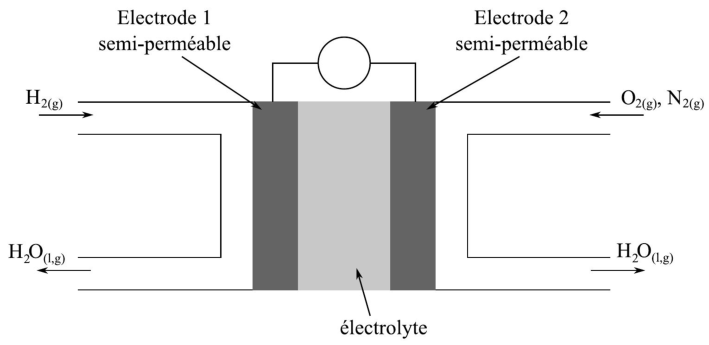
\includegraphics[width=.8\linewidth]{pile_comb}
	\captionof{figure}{Schéma de principe d'une pile à combustible.}
	\label{fig:pile_comb}
\end{center}
Chaque cellule élémentaire est constituée de deux compartiments disjoints,
alimentés chacun en gaz dihydrogène et dioxygène. Les électrodes sont séparées
par un électrolyte solide qui laisse passer les anions oxygène. Les couples
d'oxydorédution mis en jeu dans la réaction sont
$\ce{{H}^+_{\rm(aq)}/{H_2}_{\rm(g)}}$ et $\ce{{O_2}_{\rm(g)}/H_2O_{\rm(l)}}$.
}%
\QR{%
	Indiquer la position des atomes constitutifs dans les réactifs et du produit.
	En déduire les schémas de \textsc{Lewis} des trois molécules.
}{%
	solu
}%
\QR{%
	À partir des informations du schéma, attribuer et justifier le choix de la
	cathode et de l'anonde aux électrodes 1 et 2, ainsi que le sens de circulation
	des électrons.
}{%
	solu
}%
\QR{%
	Écrire les demi-équations électroniques pour chaque couple mis en jeu, quand
	la pile débite.
}{%
	solu
}%
\QR{%
	Le réactif qui est oxydé est appelé le combustible de la pile. Parmi les
	espèces chimiques présentes dans les couples, laquelle constitue le
	combustible~?
}{%
	solu
}%
\QR{%
	En déduire l'équation de la réaction modélisant la transformation ayant lieu
	dans la cellule de réaction.
}{%
	solu
}%
\enonce{%
	Dans un véhicule motorisé fonctionnant grâce à une pile à combustible, on
	estime à \SI{1.5}{kg} la masse de dihydrogène nécessaire pour parcourir
	\SI{250}{km}.
}%

\QR{%
	Calculer la quantité de matière de dihydrogène correspondant à cette masse,
	puis le volume occupé par cette quantité de gaz à $\SI{20}{\degreeCelsius}$
	sous pression atmosphérique.
}{%
	solu
}%
\QR{%
	Quel est l'avantage pour l'environnement de l'utilisation d'une pile à
	combustible au dihydrogène par rapport à un carburant classique~? Quel en est
	l'inconvénient majeur~?
}{%
	solu
}%

\resetQ
\section{Accumulateur lithium métal \hfill \small oral banque PT}
\enonce{%
	On étudie ici l'accumulateur lithium-oxyde de manganèse, qui représente
	environ 80\% du marché des batteries au lithium. La première électrode est en
	dioxyde de manganèse \ce{MnO2}, la deuxième en lithium \ce{Li}. Ces deux
	électrodes baignent dans un électrolyte organique contenant des ions \ce{Li+}.
	\begin{tcb}(data)<lfnt>{Données}
		\begin{itemize}
			\item Numéro atomique du lithium~: $Z = 3$.
			\item Masse molaire du lithium~: $M_{\ce{Li}} = \SI{5.9}{g.mol^{-1}}$.
			\item Potentiels standard~: $E_1^\circ(\ce{Li^+/Li_{\rm(s)}}) =
				      -\SI{3.03}{V}$ et
			      $E_2^\circ(\ce{{MnO_2}_{\rm(s)}/{LiMnO_2}_{\rm(s)}})$ = \SI{0.65}{V}.
		\end{itemize}
	\end{tcb}
}%
\QR{%
	Indiquer la position di lithium dans le tableau périodique. Pourquoi choisir
	un électrolyte organique plutôt que de l'eau~?
}{%
	solu
}%
\QR{%
	Écrire les réactions aux électrodes lorsque l'accumulateur fonctionne en
	générateur, ainsi que la réaction globale de fonctionnement.
}{%
	solu
}%
\QR{%
	La pile contient-elle un pont salin ou équivalent~? Pourquoi~?
}{%
	solu
}%
\QR{%
	Déterminer la force électromotrice de la pile.
}{%
	solu
}%
\QR{%
	Déterminer la capacité $C$ de la pile en \si{A.h} pour une masse initiale de
	\SI{2}{g} de lithium.
}{%
	solu
}%

\resetQ
\section{Dosage d'une solution d'hypochlorite de sodium \hfill \small écrit PT
  2016}

\enonce{%
Après avoir introduit un volume $V_0 = \SI{2.00}{mL}$ d'une solution
commerciale d'hypochlorite de sodium $(\ce{Na^+}~;~\ce{ClO^-})$ dans une fiole
jaugée de volume $V_f = \SI{100}{mL}$, on complète avec de l'eau distillée
jusqu'au trait de jauge. À un volume $V = \SI{10.0}{mL}$ de cette solutio
fille, on ajoute environ \SI{10}{mL} d'une solution d'iodure de potassium
$(\ce{K^+}~;~\ce{I^-})$ à 15\% en masse et \SI{5.0}{mL} d'acide éthanoïque
$\ce{CH_3CO_2H_{\rm(aq)}}$ à \SI{3.0}{mol.L^{-1}}. L'échantillon obtenu est
titré par une solution de thiosulfate de sodium
$(\ce{2Na^+}~;~\ce{{S_2O_3}^{2-}})$ de concentration $c =
	\SI{2.0e-2}{mol.L^{-1}}$. Le volume équivalent est égal à $V' =
	\SI{16.0}{mL}$.
\begin{tcb}(data)<lftt>{Données à \SI{298}{K}}
	\[
		E^\circ(\ce{ClO^-/Cl^-}) = \SI{0.89}{V}
		\qquad
		E^\circ(\ce{I_2/I^-}) = \SI{0.54}{V}
		\qquad
		E^\circ(\ce{{S_4O_6}^2-/{S_2O_3}^2-}) = \SI{0.08}{V}
	\]
\end{tcb}
}%
\QR{%
	Proposer une équation pour la réaction entre les ions hypochlorite
	$\ce{ClO^-}$ et les ions iodure \ce{I^-}. Prévoir qualitativement le caractère
	favorisé ou défavorisé de la réaction.
}{%
	solu
}%
\QR{%
Proposer une équation pour la réaction de titrage du diiode \ce{I2} par les
ions thiosulfate $\ce{S_2O_3^{2-}}$. Prévoir qualitativement le caractère
favorisé ou défavorisé de la réaction.
}{%
solu
}%
\QR{%
	Sachant que les ions iodure et l'acide éthanoïque sont introduits en excès,
	déterminer la concentration en ions hypochlorite dans la solution commerciale.
}{%
	solu
}%

\end{document}
